\documentclass{article}
\usepackage[utf8]{inputenc}
\usepackage[spanish]{babel}
\usepackage{listings}
\usepackage{graphicx}
\graphicspath{ {/home/mafeta/Imágenes/parcial1}}
\usepackage{cite}

\begin{document}

\begin{titlepage}
    \begin{center}
        \vspace*{1cm}
            
        \Huge
        \textbf{Análisis y Diseño Parcial 1}
            
        \vspace{0.5cm}
        \LARGE
        Sistema de encriptación 
            
        \vspace{5cm}
            
        \textbf{Maria Fernanda Tasco ALquichire}
            
        \vfill
            
        \vspace{0.8cm}
            
        \Large
        Despartamento de Ingeniería Electrónica y Telecomunicaciones\\
        Universidad de Antioquia\\
        Medellín\\
        Febrero de 2022
            
    \end{center}
\end{titlepage}

\tableofcontents
\newpage

\section{Objetivos}\label{intro}
\subsection{generales}
resumen - abstrac
\subsection{Especificos}
introducion

\section{Sección introductoria}\label{intro}
\subsection{Resumen}
resumen - abstrac
\subsection{Introdución}
introducion


\section{Marco Teorico} \label{investigación}
Esta sección es para agregar toda la información correspondiente con código, citas, etc.

\subsection{Terminología / preguntas en la investigación}
\subsubsection*{¿Qué es, para qué sirve y cómo se usa la señal de reloj?}
Una \textbf{Señal de Reloj} \cite{señal_reloj} es una señal usada para coordinar las acciones de 2 o más circuitos o sistemas. Oscila entre estado alto y bajo en forma de señal cuadrada. 
\\[0.2cm]
Es producida por un generador de reloj y usualmente empleando una frecuencia fija constante.
\\[0.2cm]
La mayoria de los circuitos integrados complejos utilizan una señal de reloj para sincronizar sus diferentes partes y controlar los tiempos de propagación.
\subsubsection*{¿74HC595?}
El circuito integrado 74HC595 es un \textbf{registro de desplazamiento} \cite{74HC595Informacion}  que cuenta con entrada en serie y salida en paralelo de 8 bits. Lo que quiere decir es que en este \textbf{tipo de registros} \cite{tipo_de_registros} con salida en paralelo se dispone de la salida de cada \textbf{flip-flop o biestable} \cite{flip-flop_o_biestable} por lo que una vez almacenados los datos cada bits se representa en su respectiva salida. Por tanto, con una sola entrada, se pueden controlar a la vez esas 8 salidas
\\[0.2cm]
Sus valores en la salida dependen de los valores de la entrada y de valores anteriores almacenados. Este registro se compone de una serie de biestables o flip-flops de tipo D comandados por una señal de reloj. Esos \textbf{biestables} \cite{flip-flop_o_biestable} son dispositivoz capaces de memorizar la información a la que antes hacía referencia. Almacena el estado 1 y 0. 
\\[0.2cm]
El desplazamiento de datos \textbf{se puede implementar} \cite{74hc595_como_funciona} utilizando puertas lógicas que permitan la transferencia de un bits de datos de una etapa a la siguiente de la izquierda o de la derecha dependiendo del nivel de una línea de control.
Dependiendo del sistema de desencriptación el circuito integrado 74hc595 nos va a ayudar a hacer un desplazamiento a la derecha o a la izquierda para coger los 8 bits que habían pasado o estaban por venir en referencia al valor para clasificar.
\\[0.2cm]
\textbf{Otra utilidad} \cite{registro_desplazamiento_almacenamiento} que tiene este CI en especial es el RCLK (Registro de reloj/Latch) Cuando este en BAJO (LOW), el contenido del registro de desplazamiento (los 8 bits) se copia en el registro de almacenamiento; que finalmente se muestra en la salida. Eso permite que mientras se realiza este proceso se puedan ir ingresando datos en serie usando el SRCLR (Shift Register Clear) que reinicia todo el registro de desplazamiento, haciendo que todos sus bits sean 0, cuando este esta en LOW y así dando paso a que el SRCLK (Shift Register Clock) que registra el cambio y desplaza los bits en el registro de desplazamiento, cuando este esta en HIGH.
\\[0.2cm]
Se puede ver la implementación de este CI con pulsadores / switches y con arduino en la sección de marco experimental.

\subsection{Investgación soluciuones propuestas}
aun no he investigado nada


\section{Marco Expremiental} \label{practica}
\subsection*{74HC595 Ejemplo de uso con pulsadores / switches}
Para esta primera implementación de ejemplo se probará el 74HC595 con un \textbf{pulsador} \cite{74hc595_pulsador} que registra los desplazamientos, otro que registra la salida y el interruptor deslizante como entrada (HIGH-LOW).

\begin{figure}[h!]
\caption{Uso 74HC595 con pulsadores en \textbf{tinkercad} \cite{ejem_74HC595_pulsadores}}
\centering
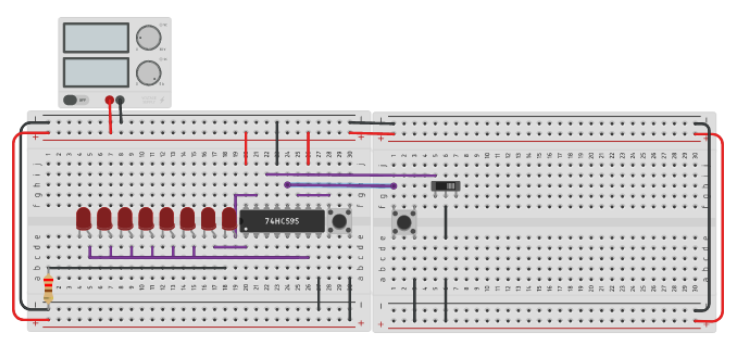
\includegraphics[width=0.5\textwidth]{ejem_75hc595_pulsadores.png}
\end{figure}

Por último se implementó el CI con arduino, en este caso colocando los 3 pines principales en los pines digitales de arduino, también se hizó uso de la función shiftOut(); de \textbf{arduino} \cite{shiftOut_arduino}

\begin{figure}[h!]
\caption{Uso 74HC595 con arduino en \textbf{tinkercad} \cite{ejem_74hc595_arduino}}
\centering
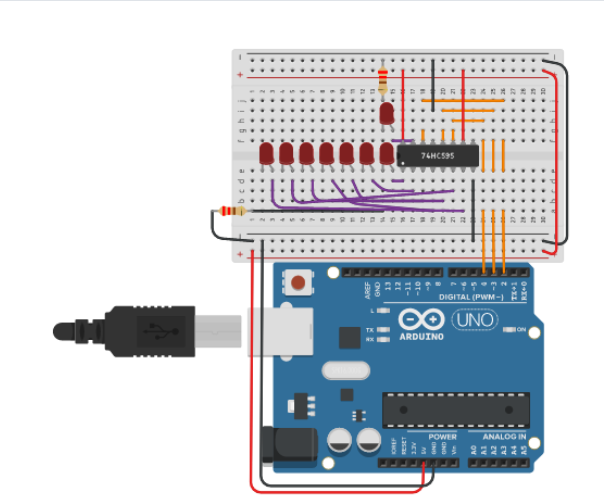
\includegraphics[width=0.5\textwidth]{Ejem_74hc595_arduino.png}
\end{figure}

con esto se concluye que 


\section{Resultados} \label{conclusiones}
Una clave para el desarrollo del algoritmo fue el orden de los pasos, ya que un orden adecuado, omitir algunos pasos o no generar las condiciones necesarias para el buen desarrollo de la solución, podría generar alguna ambigüedad o error.

\section{Conclusiones} \label{conclusiones}
Una clave para el desarrollo del algoritmo fue el orden de los pasos, ya que un orden adecuado, omitir algunos pasos o no generar las condiciones necesarias para el buen desarrollo de la solución, podría generar alguna ambigüedad o error.



(\ref{intro}), (\ref{contenido}) y (\ref{imagenes})
\bibliographystyle{IEEEtran}
\bibliography{references}

\end{document}

